\chapter{Basics}
\section{Value Networks in Industrie 4.0}
\citet[p. 6]{Sturgeon2001HowNetworks} defines value chains as the connection of value-adding activities of a company in order to create a product or a service. The activities can have complex relationships to each other and can take place at different locations. Within a company, all departments that are involved in the production or sale of a product are part of the value chain \cite[p. 10]{Sturgeon2001HowNetworks}. \citeauthor{Sturgeon2001HowNetworks} refers to this type of networking as vertical networking. Whereas the value chain focuses on the individual product, the term value network covers all value chains in which a company operates. A value network can include various cooperating as well as legally independent companies. To this end, each company within the network contributes its core competencies in order to achieve collaborative competitive advantages and create value through their mutual interaction \cite[p. 3]{Bach2010GeschaftsmodelleGrundlagen}. Consequently, value networks have in addition to the vertical networking also a horizontal networking, namely the connection across company boundaries. Value networks have therefore the potential to create new product-service bundles both, within and across companies traditional scope. Thus, companies can use value networks on the one hand to grow their existing core business, but also expand their network by tapping into new market segments \cite[p. 22]{Acatech2013Recommendations4.0}.

In the context of \ac{I4.0} especially the horizontal integration through value networks has increased. The horizontal integration is driven by the vision of autonomously acting resources within a network that can configure themselves, automatically respond to different situations, and make decisions accordingly. Horizontal networking in \ac{I4.0} is therefore almost exclusively technology-based \cite[p. 20, 21]{Acatech2013Recommendations4.0}. The control of these resources is made possible by the fact, that all relevant information is available in real-time through the networking of all instances of value creation. This enables constant evaluation and optimization of processes on the basis of the collected data in real-time \cite[p. 24]{Acatech2013Recommendations4.0}. 

The horizontal connection of partners within a value network in \ac{I4.0} is typically realized via \ac{IIOT} platforms or digital ecosystems. An \ac{IIOT} platform is characterized by the interaction of entities, information systems, business partners and people to drive production and operations in which each of the partners makes its specific added value available to other partners in the network \cite[p. 5]{Falk2020ValueChina} \cite[p. 2]{Falk2021DigitaleEntwicklung}. In the area of \ac{IIOT} platforms, two main types are emerging. Platforms, with a generic approach, that aim to collect data in general about the use and operation of spatially distributed assets in order to gain insights \cite[p. 11]{Falk2021DigitaleEntwicklung}. On the other hand, the emergence of \ac{IIOT} platforms and ecosystems around specialized offerings of companies can be seen \cite[p. 13]{Falk2021DigitaleEntwicklung}. While the former platforms predominantly take an open platform approach, the latter are mostly closed platforms. The degree of openness of a platform refers to the possibility of integrating further partners and making the platform's content accessible to them. 

A concrete use case within an \ac{IIOT} platform represents predictive maintenance. Predictive maintenance by definition refers to a maintenance process based on the evaluation of process and machine data collected by sensors \cite[p. 1670]{Selcuk2016PredictiveTrends:}. The collected data is either sent in its raw or aggregated form to the cloud, where it is stored and made available for different partner in the network. The real-time processing of the underlying data makes forecasts possible that form then the basis for needs-based maintenance. Thus, it can improve the economic efficiency of a real world asset, predict the optimal time for maintenance and improve the performance by minimizing unplanned downtime. While costs are not the only benefit of implementing predictive maintenance several other motives underlie the considerations to replace preventive maintenance by predictive maintenance. For example during agreed maintenance intervals for hardware products, most often hardware parts are replaced, although they were neither defective nor threatened to fail \cite[p. 1672]{Selcuk2016PredictiveTrends:}. A concrete example of implementation is provided by \citeauthor{Cavalieri2020AShell}. While the collection of the machine data is carried out by the operator itself, a service provider takes over the implementation of the prediction and decision model in the cloud \cite[p. 11]{Cavalieri2020AShell}.

As outlined in the case of predictive maintenance, value networks are the basis for manufacturing companies to generate new revenue streams and gain a competitive advantage, by connecting, merging and evaluating data on the use and operation of the entire product life cycle. While this example is of simple nature, value networks are often much more complex.

\begin{figure}[h]
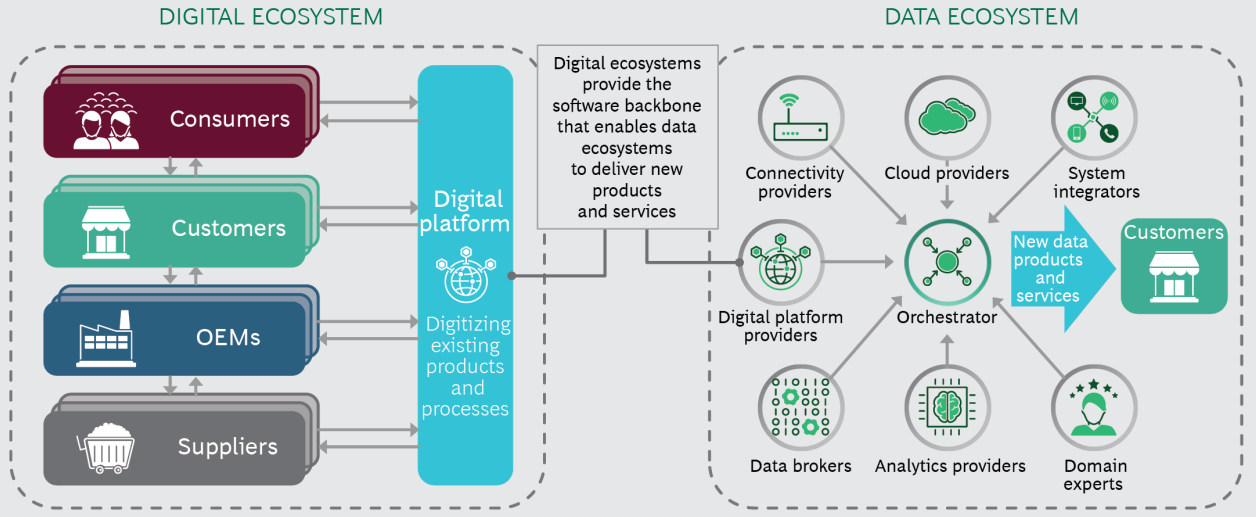
\includegraphics[scale=0.35]{content/pictures/digital_ecosystems_bcg.png}
\caption{Digital and Data Ecosystems}
\source{\cite{Russo2018HowCompetition}}
\label{fig:valuenetworksi40}
\end{figure}

Figure \ref{fig:valuenetworksi40} provides an overview of a value network in \ac{I4.0} with their roles and actors. Typically, four roles can be seen in value networks. Usually, they are identical with the players seen along the traditional value chain. These are the platform operator, the OEMs, their customers as well as suppliers. In addition to the traditional suppliers, new service providers from the digital ecosystem play an important role. Practical examples of value creation networks in \ac{I4.0} are the Airbus Skywise Platform or the Volkswagen Industrial Cloud. Skywise was launched 2017 as an internal project at Airbus with the aim of analyzing millions of data points collected during the operation of an aircraft, to get a close-up view of its condition in order to avoid defects and downtime of the aircraft to generate direct cost savings \cite{Hanke2019AirbusWerden}. Airbus has since expanded it's ambition: Skywise aims to be the leading platform for the aircraft industry to revolutionize the way aircraft are designed, built and operated by controlling the platform's key applications and architectures. To this end, Airbus has opened their platform to suppliers and service providers. This type of development is typical: First, the collected data is used to improve the company's own products, services as well as the internal processes, and in a second step an open platform is created to provide new,  data-driven products and service offers to customers 

As outlined, through \ac{I4.0} value creation networks with different companies emerge, which are characterized by complex mutual relationships. To make the complexities understandable and manageable for all partners in the value network, a common technical standard is needed. Processes and interfaces are required that define collaboration and the information to be exchanged. A reference model describes the technical description and implementation of these agreements. It thus provides a general pattern for the products and services of all cooperating companies and forms the framework for both the structuring and the development, integration and operation of the relevant technical systems. A value network consists of a wide variety of companies with different business models. The reference model has the task of bringing together the different perspectives into a common and unified view. For this purpose, it is necessary to agree on basic structuring principles as well as interfaces and data.    


\section{RAMI4.0}
\ac{RAMI4.0} is a reference model, which enables the interdisciplinary technical data description of an asset over the entire life cycle from design over production to disposal. An asset in \ac{RAMI4.0} is described as an object that has a certain business value for a company. The term therefore not only applies to physical asset but also includes ideas and software in its definition \cite[p. 31]{Heidel2017ReferenzarchitekturmodellIndustrie4.0Komponente}. \ac{RAMI4.0} is a complex model due to the variety of processes, products and services that can be mapped in it. However, when used correctly, \ac{RAMI4.0} can offer high added value in terms of the uniform mapping of technologies and asset characteristics \cite[p. 23]{Arnold2018DigitaleMittelstand}. To simplify the complex aspects and interrelationships of an asset in the context of \ac{I4.0}, \ac{RAMI4.0} consists of three dimensions: Layers, Life Cycle \& Value Stream and Hierarchy Levels. The individual dimensions are divided into sub-models to ensure that a common understanding for discussion emerges. The subdivision into sub-models makes it possible to present the relevant aspects of an asset at each point in the life cycle. Figure \ref{fig:rami40} shows the three axis of the model. 

\begin{figure}[h]
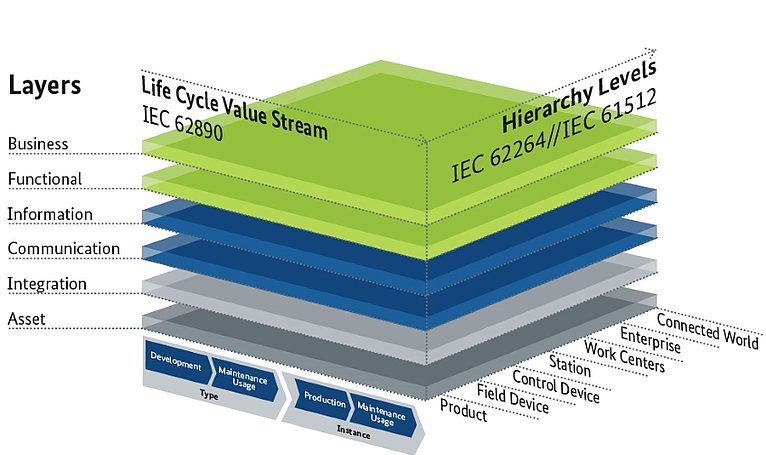
\includegraphics[scale=0.5]{content/pictures/rami_4.0_zvei.jpg}
\caption{Referenzarchitekturmodell Industry 4.0}
\source{\cite{ZVEI2015TheZvei.org}}
\label{fig:rami40}
\end{figure}

\begin{itemize}
    \item[] \textbf{Life Cycle \& Value Stream} As a result of customized products, companies are concentrating more on their core competencies and increasingly outsource value-added activities \cite[p. 11]{Arnold2018DigitaleMittelstand}. This leads to a stronger linkage and dependency of the partners in the value chain. On the Life Cycle \& Value Stream axis, these relationships of the partners in the value chain as well as the life cycle of the asset can be mapped. The life cycle of an asset is divided into type and instance \cite[p. 43]{Heidel2017ReferenzarchitekturmodellIndustrie4.0Komponente}. In the first phase of the asset, which includes the planning, development and construction of the asset, the type is created. The second phase describes the production of the previously developed asset type. The information created during production, such as material used, is added to the instance. After production, the asset is used by the customer, resulting in usage data, which is also added to the instance \cite[p. 43]{Heidel2017ReferenzarchitekturmodellIndustrie4.0Komponente}
    \item[] \textbf{Layers} The vertical axis of the architecture model describes the structural properties of an asset or their combination in six layers. The lowest layer is the \textit{Asset-Layer}. It represents the real asset in the physical world. All superordinate layers are to be assigned to the information world \cite[p. 46]{Heidel2017ReferenzarchitekturmodellIndustrie4.0Komponente}. The \textit{Integration-Layer} connects the physical world with the virtual world by transferring generated events of the physical world (for example, the change of the state of a machine) into the virtual world \cite[p. 47]{Heidel2017ReferenzarchitekturmodellIndustrie4.0Komponente}. The communication layer describes the access to the asset's information. This includes the protocol to use, the data format and the transmission of the data. The ensure interoperability the protocol and data format must be according to \ac{I4.0} standards. This allows assets from different layers and networks to connect to each other \cite[p. 47,48]{Heidel2017ReferenzarchitekturmodellIndustrie4.0Komponente}. The provision of the structured data, the processing of the events sent by the asset and analysis of these take place in the \textit{Information-Layer} \cite[p. 51]{Heidel2017ReferenzarchitekturmodellIndustrie4.0Komponente}. Services, capabilities and functions provided by the asset are mapped in the \textit{Functional-Layer} \cite[p. 51]{Heidel2017ReferenzarchitekturmodellIndustrie4.0Komponente}. Within the function layer, a distinction is made between basic, process and manufacturer-specific functions. Basic functions are manufacturer-independent functions that base their functionality on \ac{I4.0} compliant data from the information layer. One example for this is predictive maintenance. Process functions on the other hand are production specific such as forming or cutting. Manufacturer-specific functions are those that are not \ac{I4.0} compliant and are proprietary. \textit{Business-Layer} describes the business processes and is responsible for orchestrating the services defined in the functional layer. It thus maps the business models and the resulting overall processes \cite[p. 53]{Heidel2017ReferenzarchitekturmodellIndustrie4.0Komponente}.
    \item[] \textbf{Hierarchy Levels} This axis refers to the functional classification within an \ac{I4.0} factory and ranges from product to technical plant to the networked world.
\end{itemize}

\section{Digital Twin}



